% Template Header
\documentclass[12pt]{article}
\usepackage{graphicx}
\graphicspath{{./images/}}
\usepackage[a4paper,margin=15mm]{geometry}
\usepackage[table]{xcolor}
%\usepackage{xcolor}
\usepackage{tikz}
\usepackage{lastpage}
\usepackage{fancyhdr}
\usepackage{hyperref}

%\usepackage{atbegshi,etoolbox}

\renewcommand{\familydefault}{\sfdefault}

\parskip 7.2pt

\def\doctitle{Kinova MoveIt Development Report}
\def\docauthor{Longfei Zhao}
\def\docdate{\today}
\def\docrevision{(Revision 01)}
\def\doctype{X?.?-01\_Documentation R01}
\def\docconfidentiality{CONFIDENTIAL - ROS MoveIt}
\def\docfilename{Kinova-Moveit-Report.pdf}

\hypersetup{
    colorlinks,
    citecolor=black,
    filecolor=black,
    linkcolor=black,
    urlcolor=black
}
% End Template Header

\usepackage[cmex10]{amsmath}
\usepackage{multirow}
\usepackage{makecell}
\usepackage{soul}
\usepackage{array}
\usepackage{color}
\usepackage{transparent}
%% Utilisation de natbib pour les citations et la bibliographie.
\usepackage{natbib}
%% Autres packages.
\usepackage{amsmath,color,soulutf8,longtable,colortbl,setspace,ifthen,xspace,url,pdflscape}



%\newif\ifkeeppage
%\newcommand{\keeppages}[1]{% \keeppages{<csv list>}
%	\xdef\keep@pages{#1}% Store pages to keep
%	\AtBeginShipout{% At shipout, decide whether to discard page/not
%		\keeppagefalse%
%		\renewcommand*{\do}[1]{% How to handle each page entry in csv list
%			\ifnum\value{page}=##1\relax%
%			\keeppagetrue% Page should be kept
%			\gdef\do####1{}% Do nothing further
%			\fi%
%		}%
%		\expandafter\docsvlist\expandafter{\keep@pages}% Process list of pages to keep
%		\ifkeeppage\else\AtBeginShipoutDiscard\fi% Discard page/not
%	}%
%}
%\makeatother
%
%\keeppages{3}

\begin{document}

% To use this cover, you need to have the following in your preamble
%
% \documentclass[12pt]{article}
% \usepackage{graphicx}
% \usepackage[a4paper,margin=15mm]{geometry}
% \usepackage[table]{xcolor}
% \usepackage{tikz}
% \usepackage{lastpage}
% \usepackage{fancyhdr}
%
% And you need to define these parameters:
%
% \def\doctitle{TITLE}
% \def\docauthor{AUTHOR}
% \def\docdate{DATE}                % Note: \today could be used for DATE
% \def\docrevision{REVISION}        % For example `Revision 01`
% \def\doctype{TYPE}                % For example `F7.3-02_Product Requirement R01`
% \def\docconfidentiality{CONF}     % For example `Internal Use Only`, or `Confidential`
% \def\docfilename{FILENAME}
%
% This cover was designed with this family of fonts, and may be out of shape with a different font:
%
% \renewcommand{\familydefault}{\sfdefault}
%
% The Kinova logo must be present in images/logo_kinova.pdf, and a version with
% white font instead of black, in images/logo_kinova_inv.pdf.
% If you have an svg, you can convert it first to eps with Inkscape:
%
%     inkscape file.svg --export-eps=file.eps
%
% and then from eps to pdf:
%
%     epstopdf --outfile=file.pdf file.eps
%
% To use this cover, after \begin{document}, simply do:
%
%     % To use this cover, you need to have the following in your preamble
%
% \documentclass[12pt]{article}
% \usepackage{graphicx}
% \usepackage[a4paper,margin=15mm]{geometry}
% \usepackage[table]{xcolor}
% \usepackage{tikz}
% \usepackage{lastpage}
% \usepackage{fancyhdr}
%
% And you need to define these parameters:
%
% \def\doctitle{TITLE}
% \def\docauthor{AUTHOR}
% \def\docdate{DATE}                % Note: \today could be used for DATE
% \def\docrevision{REVISION}        % For example `Revision 01`
% \def\doctype{TYPE}                % For example `F7.3-02_Product Requirement R01`
% \def\docconfidentiality{CONF}     % For example `Internal Use Only`, or `Confidential`
% \def\docfilename{FILENAME}
%
% This cover was designed with this family of fonts, and may be out of shape with a different font:
%
% \renewcommand{\familydefault}{\sfdefault}
%
% The Kinova logo must be present in images/logo_kinova.pdf, and a version with
% white font instead of black, in images/logo_kinova_inv.pdf.
% If you have an svg, you can convert it first to eps with Inkscape:
%
%     inkscape file.svg --export-eps=file.eps
%
% and then from eps to pdf:
%
%     epstopdf --outfile=file.pdf file.eps
%
% To use this cover, after \begin{document}, simply do:
%
%     % To use this cover, you need to have the following in your preamble
%
% \documentclass[12pt]{article}
% \usepackage{graphicx}
% \usepackage[a4paper,margin=15mm]{geometry}
% \usepackage[table]{xcolor}
% \usepackage{tikz}
% \usepackage{lastpage}
% \usepackage{fancyhdr}
%
% And you need to define these parameters:
%
% \def\doctitle{TITLE}
% \def\docauthor{AUTHOR}
% \def\docdate{DATE}                % Note: \today could be used for DATE
% \def\docrevision{REVISION}        % For example `Revision 01`
% \def\doctype{TYPE}                % For example `F7.3-02_Product Requirement R01`
% \def\docconfidentiality{CONF}     % For example `Internal Use Only`, or `Confidential`
% \def\docfilename{FILENAME}
%
% This cover was designed with this family of fonts, and may be out of shape with a different font:
%
% \renewcommand{\familydefault}{\sfdefault}
%
% The Kinova logo must be present in images/logo_kinova.pdf, and a version with
% white font instead of black, in images/logo_kinova_inv.pdf.
% If you have an svg, you can convert it first to eps with Inkscape:
%
%     inkscape file.svg --export-eps=file.eps
%
% and then from eps to pdf:
%
%     epstopdf --outfile=file.pdf file.eps
%
% To use this cover, after \begin{document}, simply do:
%
%     \input{kinovacover.tex}
%

\begin{titlepage}

  \vspace*{10mm}
  \begin{center}
    \Huge{\textbf{\doctitle}}

    \vspace*{15mm}
    \Large{\textbf{\docrevision}}

    \Large{\textbf{\docdate}}

    \vspace*{15mm}
    \textbf{By}

    \Large{\textbf{\docauthor}}
  \end{center}

  \vspace*{10mm}
  \hspace{-5cm}
  
\begin{tikzpicture}
    \draw[color=black,fill=black] (0,0) rectangle (50cm,5.5cm);
    \draw[color=cyan,fill=cyan] (0,5.5cm) rectangle (50cm,6cm);
  \end{tikzpicture}

  \vspace*{-50mm}

  \begin{center}
    
\includegraphics[width=10cm]{images/logo_kinova_inv}
  \end{center}

  \vspace*{20mm}
  \noindent
  \textbf{Warning}

  \noindent
  The information contained in this document is the property of Kinova. Except as
  specifically authorized in writing by Kinova, the holder of this document shall keep the
  information contained here confidential and shall protect same in whole or in part from
  disclosure and dissemination to third parties and use same for evaluation, operation and
  maintenance purposes only. This document is not an engagement of Kinova to develop,
  implement or design the product or techniques described here.

\end{titlepage}

\newpage

\setlength{\voffset}{-1in}
\setlength{\topmargin}{10pt}
\setlength{\headheight}{50pt}
\setlength{\footskip}{40pt}
\setlength{\textheight}{0.9\textheight}
\pagestyle{fancy}
\fancyhf{}
\fancyhead[L]{\color{gray}{\renewcommand{\arraystretch}{0.75}\begin{tabular}{l}
    \footnotesize \doctype - \doctitle \\
    \footnotesize Effective Date: \docdate \\
    \footnotesize \textbf{\docconfidentiality} \\
  \end{tabular}}
}
\fancyhead[R]{\includegraphics[width=40mm]{images/logo_kinova}\vspace*{-15pt}}
\renewcommand{\headrulewidth}{0.5pt}
\fancyfoot[L]{\vspace*{-7pt}\color{gray}{\renewcommand{\arraystretch}{0.75}\begin{tabular}{l}
    \footnotesize \docfilename \\
    \footnotesize Printed: \docdate \\
  \end{tabular}}
}
\fancyfoot[R]{\footnotesize Page \thepage~of \pageref{LastPage}}
\renewcommand{\footrulewidth}{0.5pt}

%

\begin{titlepage}

  \vspace*{10mm}
  \begin{center}
    \Huge{\textbf{\doctitle}}

    \vspace*{15mm}
    \Large{\textbf{\docrevision}}

    \Large{\textbf{\docdate}}

    \vspace*{15mm}
    \textbf{By}

    \Large{\textbf{\docauthor}}
  \end{center}

  \vspace*{10mm}
  \hspace{-5cm}
  
\begin{tikzpicture}
    \draw[color=black,fill=black] (0,0) rectangle (50cm,5.5cm);
    \draw[color=cyan,fill=cyan] (0,5.5cm) rectangle (50cm,6cm);
  \end{tikzpicture}

  \vspace*{-50mm}

  \begin{center}
    
\includegraphics[width=10cm]{images/logo_kinova_inv}
  \end{center}

  \vspace*{20mm}
  \noindent
  \textbf{Warning}

  \noindent
  The information contained in this document is the property of Kinova. Except as
  specifically authorized in writing by Kinova, the holder of this document shall keep the
  information contained here confidential and shall protect same in whole or in part from
  disclosure and dissemination to third parties and use same for evaluation, operation and
  maintenance purposes only. This document is not an engagement of Kinova to develop,
  implement or design the product or techniques described here.

\end{titlepage}

\newpage

\setlength{\voffset}{-1in}
\setlength{\topmargin}{10pt}
\setlength{\headheight}{50pt}
\setlength{\footskip}{40pt}
\setlength{\textheight}{0.9\textheight}
\pagestyle{fancy}
\fancyhf{}
\fancyhead[L]{\color{gray}{\renewcommand{\arraystretch}{0.75}\begin{tabular}{l}
    \footnotesize \doctype - \doctitle \\
    \footnotesize Effective Date: \docdate \\
    \footnotesize \textbf{\docconfidentiality} \\
  \end{tabular}}
}
\fancyhead[R]{\includegraphics[width=40mm]{images/logo_kinova}\vspace*{-15pt}}
\renewcommand{\headrulewidth}{0.5pt}
\fancyfoot[L]{\vspace*{-7pt}\color{gray}{\renewcommand{\arraystretch}{0.75}\begin{tabular}{l}
    \footnotesize \docfilename \\
    \footnotesize Printed: \docdate \\
  \end{tabular}}
}
\fancyfoot[R]{\footnotesize Page \thepage~of \pageref{LastPage}}
\renewcommand{\footrulewidth}{0.5pt}

%

\begin{titlepage}

  \vspace*{10mm}
  \begin{center}
    \Huge{\textbf{\doctitle}}

    \vspace*{15mm}
    \Large{\textbf{\docrevision}}

    \Large{\textbf{\docdate}}

    \vspace*{15mm}
    \textbf{By}

    \Large{\textbf{\docauthor}}
  \end{center}

  \vspace*{10mm}
  \hspace{-5cm}
  
\begin{tikzpicture}
    \draw[color=black,fill=black] (0,0) rectangle (50cm,5.5cm);
    \draw[color=cyan,fill=cyan] (0,5.5cm) rectangle (50cm,6cm);
  \end{tikzpicture}

  \vspace*{-50mm}

  \begin{center}
    
\includegraphics[width=10cm]{images/logo_kinova_inv}
  \end{center}

  \vspace*{20mm}
  \noindent
  \textbf{Warning}

  \noindent
  The information contained in this document is the property of Kinova. Except as
  specifically authorized in writing by Kinova, the holder of this document shall keep the
  information contained here confidential and shall protect same in whole or in part from
  disclosure and dissemination to third parties and use same for evaluation, operation and
  maintenance purposes only. This document is not an engagement of Kinova to develop,
  implement or design the product or techniques described here.

\end{titlepage}

\newpage

\setlength{\voffset}{-1in}
\setlength{\topmargin}{10pt}
\setlength{\headheight}{50pt}
\setlength{\footskip}{40pt}
\setlength{\textheight}{0.9\textheight}
\pagestyle{fancy}
\fancyhf{}
\fancyhead[L]{\color{gray}{\renewcommand{\arraystretch}{0.75}\begin{tabular}{l}
    \footnotesize \doctype - \doctitle \\
    \footnotesize Effective Date: \docdate \\
    \footnotesize \textbf{\docconfidentiality} \\
  \end{tabular}}
}
\fancyhead[R]{\includegraphics[width=40mm]{images/logo_kinova}\vspace*{-15pt}}
\renewcommand{\headrulewidth}{0.5pt}
\fancyfoot[L]{\vspace*{-7pt}\color{gray}{\renewcommand{\arraystretch}{0.75}\begin{tabular}{l}
    \footnotesize \docfilename \\
    \footnotesize Printed: \docdate \\
  \end{tabular}}
}
\fancyfoot[R]{\footnotesize Page \thepage~of \pageref{LastPage}}
\renewcommand{\footrulewidth}{0.5pt}


\parindent = 0pt

\tableofcontents

\newpage

\section{Introduction}
The Kinova robot uses a PID loop in its actuator to control its movement. However, the robot can show visible vibrations in some conditions, mainly due to the flexibility of the robot and the mechanical properties of the harmonic drive used in the actuator, that can not be compensated by the PID loop alone. For that purpose, a torque feedback loop is implemented in the four biggest actuators of the MS5-6 Rev2c arms. From the solutions tried at Kinova to damp vibrations, using a torque compensation based on torque measurements (strain gages) and feeding it to the actuator gives the best results.

This document describes the torque feedback loop used, gives details on the compensator transfer function, shows actual performance enhancement results obtained from testing, and discuss both ongoing and future works on MS5-6 Rev2c and MS7 arms.

%This document describes the torque feedback loop used and shows actual performance enhancement results obtained from testing. Please keep in mind that this document is a preliminary version aimed at showing available results alone.

A document titled "Kinova Actuator Controller" has also been provided. It contains a detailed description of the control loop, including PID control, BEMF compensation, friction compensation, torque feedback, etc. The reader is therefore referred to this document if more details on the control loop are required.




\newpage

\section{Torque Feedback Loop}
The basic control loop of the controller is shown in fig.~\ref{fig:loop}. One can see that a torque measurement is fed into a torque compensator, multiplied by a gain $K_{\tau}$ and added to the PID output to the actuator. The compensator has 7 poles and 7 zeros. Please note that no additional filtering is applied before or after that compensator. In other words, the torque measurement, i.e. the mean value of the 8 strain gages, is directly taken as input to the compensator and the output is itself fed to the actuator through simple gain $K_\tau$. The torque measurement are refreshed each 7~milliseconds, therefore the torque loop runs at 143Hz. The $z$-transform of the compensator transfer function is:
\begin{align}
	\tau_f = K_{B\tau}\frac{b_1 + b_2z^{-1} + b_3z^{-2} + \cdots + b_8z^{-7}}{a_1 + a_2z^{-1} + a_3z^{-2} + \cdots + a_8z^{-7}}, \label{eqn:tf}
\end{align}
where $\tau_f$ is the output of the compensator and $K_{B\tau}$ is the gain of the compensator. Parameters $a_1$ to $a_8$ and $b_1$ to $b_8$ can be tuned to obtain desired zeros and poles respectively. The implementation in the firmware is straightforward:
\begin{align}
	\tau_{f_k} = \frac{1}{a_1}[K_{B\tau}(b_1\tau_k+b_2\tau_{k-1}+b_3\tau_{k-2}+\cdots+b_8\tau_{k-7})-(a_2\tau_{f_{k-1}}+a_3\tau_{f_{k-2}}+\cdots+a_8\tau_{f_{k-7}})] \label{eqn:firmware},
\end{align}
where $k$ is the current step.

	\begin{figure}
		\begin{center}
			\def\svgwidth{173mm}%.75\textwidth
			\input{./images/loop2.pdf_tex}
			\caption{Basic PID control loop with torque feedback}
			\label{fig:loop}
		\end{center}
	\end{figure}

Please note that in reality, torque is measured in the opposite direction compared to position, and therefore, in the actuator firmware, torque feedback is fed as a positive value to avoid negative gains. See the more detailed documentation "Kinova Actuator Controller" for details.


\newpage

%\section{Torque Compensator}
%The objective pursued when developing torque compensation is to damp vibration. However, it shall not do so while adversely affecting position tracking. Therefore, gain should be small for the required control bandwidth (up to 5Hz). Moreover, since the torque signal is not filtered, the gain at high frequencies should be low to avoid noise amplification. Since vibration is observed when resonance occurs at the robot natural frequency, the compensator could only let pass through a frequency range covering the problematic configurations corresponding frequencies. Moreover, stability issues limit the gain of the compensator.

As a consequence of the aforementioned reasons, the torque compensator transfer function is designed as a bandpass filter. However, the bandpass is really narrow and the gain is small. The transfer function is defined by the parameters listed in table~\ref{table:compensator} and eq.~\ref{eqn:tf}. The bode plot of the transfer function, including torque feedback gain $K_{\tau}$, is shown in fig.~\ref{fig:bodeComp}. Poles of the continuous transfer function in the root locus are shown in fig.~\ref{??} ?? and discrete ones are shown in fig.~\ref{??}. Poles are listed in table~\ref{??}.

\begin{table}[t]
	\caption{Vibration damping - torque compensator parameters}
	\centering                                                                      
	\hfill \break??
	\begin{tabular}{c|c||c|c}                                                
		\hline                                                                          
		Parameter & Value & Parameter & Value \\
		\hline
		$b_1$ & 0.015000 & $a_1$ & 1.000000  \\
		\hline
		$b_2$ & -0.027294 & $a_2$ & -3.153210 \\
		\hline
		$b_3$ & 0.009323 & $a_3$ & 3.807353 \\
		\hline
		$b_4$ & 0.005669 & $a_4$ & -2.084253 \\
		\hline
		$b_5$ & -0.002623 & $a_5$ & 0.435096 \\
		\hline
		$b_6$ & 0 & $a_6$ & 0 \\
		\hline
		$b_7$ & 0 & $a_7$ & 0 \\
		\hline
		$b_8$ & 0 & $a_8$ & 0 \\
		\hline
		$K_b$ & 1 & $K_{\tau}$ & 1.5 \\
		\hline
	\end{tabular}
	\label{table:compensator}
\end{table}

	\begin{figure}
		\begin{center}
			\def\svgwidth{.75\textwidth}%.75\textwidth
			\input{./images/bodePlotComp.pdf_tex}
			\caption{Torque compensator transfer function bode plot (including $K_{\tau}$)}
			\label{fig:bodeComp}
		\end{center}
	\end{figure}


%\section{Test Method}
%The robot end effector is moved back and forth between two points along a diagonal in the robot workspace, see fig.~\ref{fig:path}. The trajectory is from XYZ (0.5,-0.5,0.45) to (0.25,0.6,-0.1) in meters and is repeated 9 times. Optitrack camera system is used to track the end effector. The test is performed at 30 mm/s and 50 mm/s on two different robots. Tests at 50 mm/s (above maximal nominal speed) show more vibration and better demonstrate the vibration damping from torque feedback.

\begin{figure}
	\begin{center}
	\includegraphics[width=.8\textwidth]{./images/testPath.jpg}%
		\caption{Test Trajectory}
	\label{fig:path}
	\end{center}
\end{figure}

From previous tests, vibration frequencies are known to be above 5~Hz. Therefore, a high-pass filter at 1~Hz is applied on the collected data to isolate vibration.  The mean, standard and maximum deviations are computed from it. Filtered data from two parts (over the 9) of the trajectory are shown in fig.~\ref{fig:data}. Regions of the trajectory showing worst behavior in terms of vibration are isolated and the same (but local) analysis is performed, see enclosed regions in fig.~\ref{fig:data}. All results are shown in table~\ref{table:results_torque}.

\begin{figure}
	\begin{center}
			\includegraphics[width=1\textwidth]{./images/data2.pdf}%
			\caption{Filtered data from 2 parts of the trajectory and selected region for local analysis - Errata mm should be m}
			\label{fig:data}
	\end{center}
\end{figure}

%\section{Test Results}
%%Tests Results
%\begin{table}[t]                                                               
%	\caption{Torque feedback for vibration damping - Results}
%	\centering                                                                      
%	\hfill \break
%	\begin{tabular}{cc|ccc|ccc}                                                
%		\hline                                                                          
%		Velocity [mm/s] & \thead{Torque\\Feedback} & \multicolumn{3}{c|}{Arm \#xx} & \multicolumn{3}{c}{Arm \#xx2} \\ %\multirow{3}{*}{\thead{Velocity\\[mm/s]}} \thead{Torque\\Feedback} \thead{Velocity\\[mm/s]}
%		\hline
%		& & \multicolumn{6}{c}{Deviation [mm]} \\
%		& & mean & std & max & mean & std & max \\
%		\hline
%	    \multirow{2}{*}{30} & off & M & S & M & M & S & M \\
%		  & on & M & S & M & M & S & M \\
%		\hline
%			    \multirow{2}{*}{30*} & off & M & S & M & M & S & M \\
%			    & on & M & S & M & M & S & M \\
%			    \hline
%	   \multirow{2}{*}{50} & off & M & S & M & M & S & M \\
%	   & on & M & S & M & M & S & M \\
%	   \hline
%	   	   \multirow{2}{*}{50*} & off & M & S & M & M & S & M \\
%	   	   & on & M & S & M & M & S & M \\
%	   	   \hline
%	\end{tabular}
%	\label{table:results_torque}
%\end{table}

Test results are shown in table~\ref{table:results_torque}. The superscript "*" on the velocity specifies the results from the analysis on the selected regions of the trajectory showing most of the vibration. There is a significant reduction of vibration amplitude for tests performed at 50~mm/s. The presence of vibration over a biggest part of the trajectory and higher torque measurements due to the higher speed explains these results compared to trajectories performed at 30~mm/s. Moreover, no significant improvement is observed for arm PJ~00090~00009~16145~0001 at 30~mm/s. However, the maximum deviation is still reduced and contained under 1.5~mm for all tests.

Compared to the preliminary results shown in April 2016 in a presentation titled "7-DOF Arm – Vibration Investigation", smaller improvements on vibration reduction are observed from the current analysis. The major factor explaining this is the modification of the torque compensator, mainly due to stability issues. Compensator transfer function was modified to stabilize the torque loop in some configurations. Moreover, in April, the tests were performed at a constant joint speed (on joint 2 alone) instead of using a Cartesian trajectory therefore using all joints at the same time.

\begin{table}[t]
	\centering
	\caption{Torque feedback for vibration damping - Results}
	\includegraphics[width=.8\textwidth]{./images/Results.pdf}
	\label{table:results_torque}
\end{table}

To illustrate the effect of the torque feedback, the robot was hit in two direction and the following vibration was registered using the Optitrack system. The configuration of the robot and the direction of the hits are shown in fig.~\ref{fig:hitConfig}. On fig.~?? to ??, one can observe the natural frequency damping performed by the torque feedback compared to data collected when torque feedback is deactivated. 

\begin{figure}
	\begin{center}
		\includegraphics[width=1\textwidth]{./images/naturalVib.pdf}%
		\caption{Natural frequency damping test configuration}
		\label{fig:hitConfig}
	\end{center}
\end{figure}

%\section{Stability Analysis}
%The current section present the work done on the stability analysis of the torque feedback. This is an ongoing work and here are presented preliminary results obtained as for now. Please keep in mind that all information contained here is subject to change.

In the current robot architecture, position $\theta$, commanded position  $\theta_d$ are sampled at 1~ms, while torque $\tau_f$ is refreshed approximately each 7~ms and command $u$ at 11~ms. These are the four main outputs usable for frequency response analysis, see fig.~\ref{fig:loop}. Therefore, data analysis has to be performed with these available data.

%\begin{figure}
%	\begin{center}
%		\def\svgwidth{173mm}%.75\textwidth
%		\input{./images/loop.pdf_tex}
%		\caption{Basic PI-D control loop with torque feedback}
%		\label{fig:loop}
%	\end{center}
%\end{figure}


%\subsection{Producing bode plots}\label{sec:bode}

%\subsection{Torque Loops}\label{sec:bode}
To trace a bode plot of the torque open loop, one needs the input $u$ and the output $\tau_c$, see fig.~\ref{fig:loop}. Output of the torque loop is computed from the output of the torque compensator:
\begin{align}
\tau_c &= K_{\tau}\tau_f. \label{eqn:tauc}
\end{align}

Previously, command $u$ was not considered usable for data analysis due to its slow refresh rate, i.e. 11~ms. The signal was thereby computed from position command $\theta_d$ and position feedback $\theta$. However, the command is logged before it is sent to the actuator. Difficulties in synchronizing in time the feedback information communicated by the actuator to the corresponding command led to a significant overestimation of the position error $\theta_{err}$ and therefore command $u$. In consequence, input of the torque open loop was overestimated and hence, the gain of the open loop was underestimated. The task of synchronizing these value was found not to be straight forward, justifying the use of the slowly refreshed command $u$.

As described in document "Kinova Actuator Controller", command sent to the motor is subject to clamping based on velocity and temperature. The measurement of the command is made after those limitation are applied. Therefore, if the clamping is considered part of the plant, since it is fixed by mechanical constraints and not subject to change, $u$ can be smaller than the actual output of the PID and the torque loop combined and can lead to an underestimation of the command sent by the controler. That could make an overestimation of the gain of the open loop and hence a underestimation of the gain and phase margin, i.e. worst margins than expected. However, in the frequency responses performed for the current analysis, command $u$ mostly remained under the limitation imposed, especially in the frequency range were the stability margins are observed.


\subsection{Test Method}

\begin{itemize}
	\item Sine-swept
	
	Due to the current firmware limitations, frequency responses can be performed using position inputs only. It is known that this is not ideal to perform stability analysis of the torque loop. Moreover, having the position loop active affect the results.
	
	The sine-swept is sent accordingly to the following equation: ??
	
	Tested range of frequency is from 0 to 38Hz. To prevent damage to the robot, for each configuration, a first test covering the whole range of frequency is performed with a small half-amplitude of 0.05~deg. In a second test, the half-amplitude is raised to 0.1~deg and the frequency range is limited to where margins are observed.
	
	\item Test setup
	
	To perform frequency responses, the robot is attached to an aluminum bed with a steel plate of 1/2 inch. Therefore, flexibility of the bed, the steel plate and even the movement of the bed relative to the ground affect results. A picture of the test setup is shown in fig.~\ref{fig:bed}.
	
	\item End effector mass
	
	Assuming that the arm is used in operation with an IDM, a mass is attached to the robot for all frequency responses performed to obtain the data presented in the current document. The mass of the end effector is 1.3~kg.
	
	\item Configuration tested
	
	To perform a broad analysis, yet without performing an unnecessary large number of tests, a set of configurations covering a range over joint 2 and joint 4 is used. These joints are known to be affecting inertia the most. Moreover, a set of clinical arm configurations have been sent previously to Kinova for maximum insertion and retraction force. Since they represent normal operation configurations, they have been tested too. However, the joint 1 angle has been modified for each configuration to keep the arm above the test bed. The basic configuration and the 10 clinical cases are presented in table~\ref{table:cases}.

	

\end{itemize}

	\begin{table}[t]
		\centering
		\caption{Stability analysis: tested configurations}
		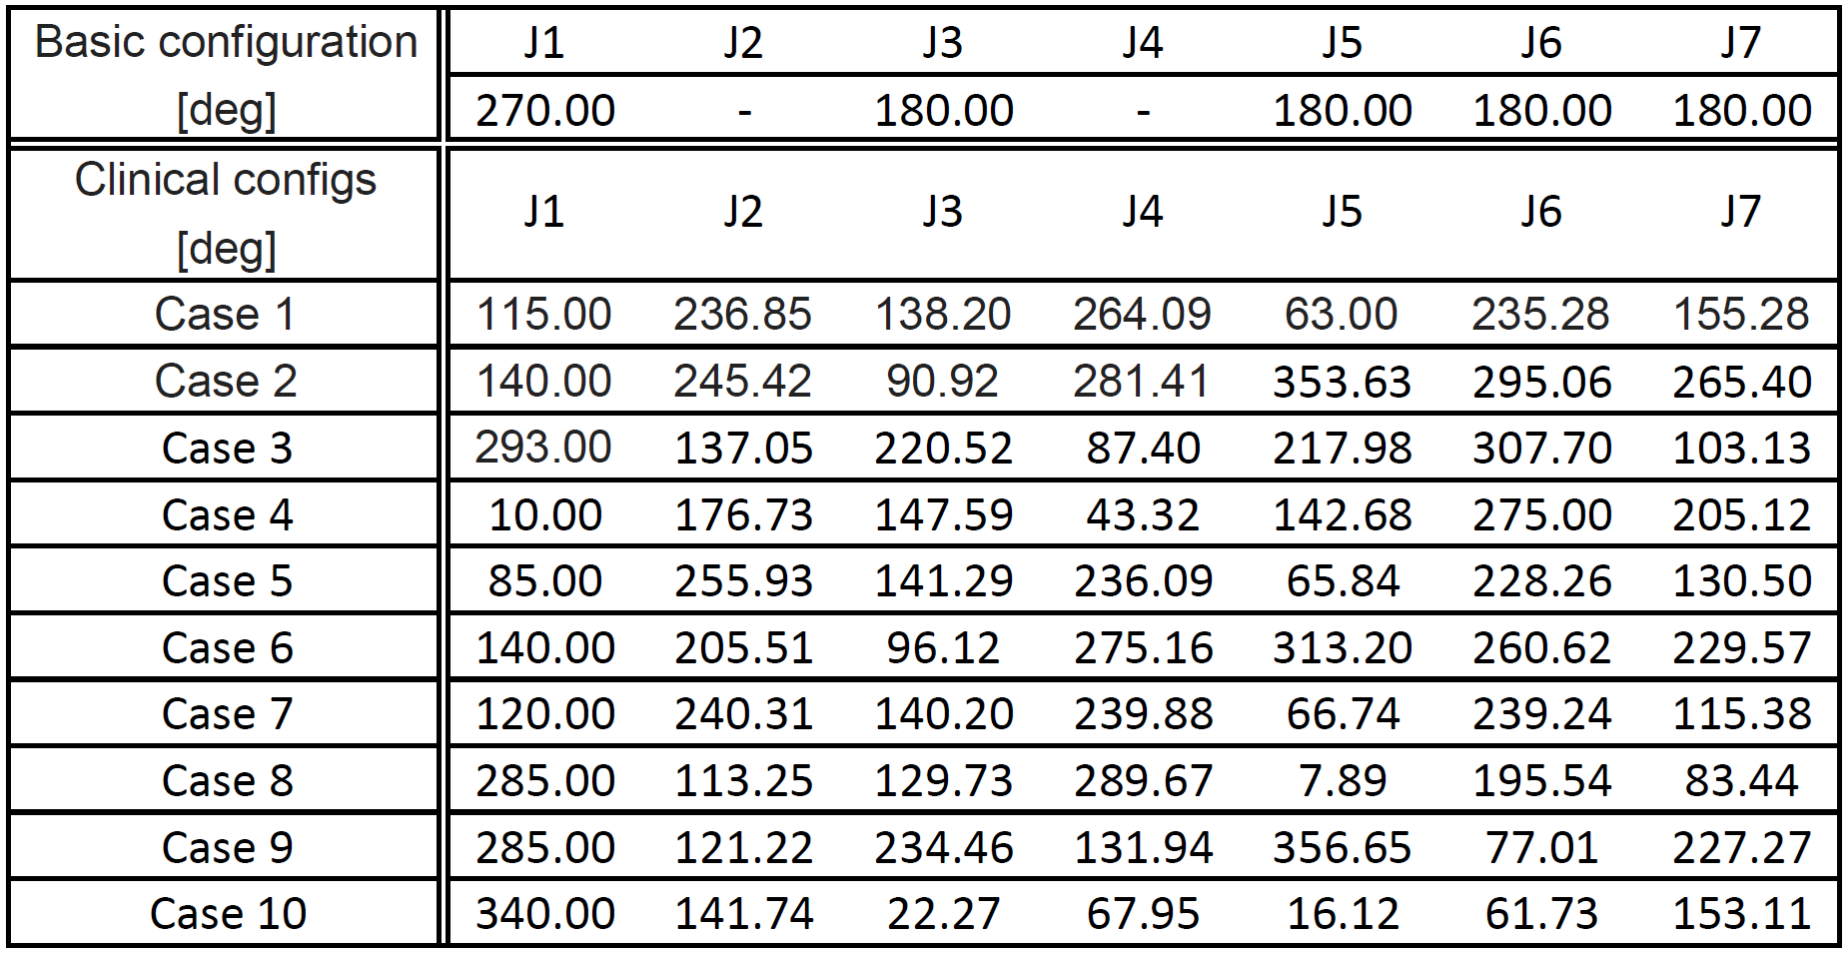
\includegraphics[width=.8\textwidth]{./images/configs.pdf}%
		%		\includegraphics[width=0.5\textwidth]{./images/test_setup_2.JPG}%
		% test_setup
		\label{table:cases}
	\end{table}

\begin{figure}
	\begin{center}
		%\begin{table}[t]
		%	\centering
		\includegraphics[width=1\textwidth]{./images/bed.jpg}%
		\caption{Test setup for frequency responses}
		\label{fig:bed}
		%\end{table}
	\end{center}
\end{figure}


%The robot end effector is moved back and forth between two points along a diagonal in the robot workspace, see fig.~\ref{fig:path}. The trajectory is from XYZ (0.5,-0.5,0.45) to (0.25,0.6,-0.1) in meters and is repeated 9 times. Optitrack camera system is used to track the end effector. The test is performed at 30 mm/s and 50 mm/s on two different robots. Tests at 50 mm/s (above maximal nominal speed) show more vibration and better demonstrate the vibration damping from torque feedback.

\begin{figure}
	\begin{center}
	\includegraphics[width=.8\textwidth]{./images/testPath.jpg}%
		\caption{Test Trajectory}
	\label{fig:path}
	\end{center}
\end{figure}

From previous tests, vibration frequencies are known to be above 5~Hz. Therefore, a high-pass filter at 1~Hz is applied on the collected data to isolate vibration.  The mean, standard and maximum deviations are computed from it. Filtered data from two parts (over the 9) of the trajectory are shown in fig.~\ref{fig:data}. Regions of the trajectory showing worst behavior in terms of vibration are isolated and the same (but local) analysis is performed, see enclosed regions in fig.~\ref{fig:data}. All results are shown in table~\ref{table:results_torque}.

\begin{figure}
	\begin{center}
			\includegraphics[width=1\textwidth]{./images/data2.pdf}%
			\caption{Filtered data from 2 parts of the trajectory and selected region for local analysis - Errata mm should be m}
			\label{fig:data}
	\end{center}
\end{figure}


\subsection{Data Analysis}
\begin{itemize}
	\item Matlab ??
\end{itemize}

\subsection{Preliminary Results}

Margins computed from the frequency responses are shown in table~\ref{table:SAtable}. According to those results, torque open loop is mainly unstable or close to instability. However, no instability is observed in operation. The whole controller is therefore most likely to be stable, i.e. position and torque closed loop running at the same time. However, open loops should show acceptable stability margins. Unfortunately, actual torque feedback parameters were set before the completion of the current analysis and previous frequency responses analysis were underestimating the gain.

Since most margins are observed around the same frequencies, namely around 13~Hz, more than simply reducing gains, i.e. modification of the torque compensator, reducing phase lag at that frequency for example, could help in stabilizing the torque loop. Open loop gain can also vary significantly between two configurations. Gain scheduling could therefore offer better performance and stability.

Typical bode plots of the torque open loop are shown in fig.??. One can notice that the frequency response can vary significantly from one configuration to the other and for one actuator to the other. Torque loops could benefit from different compensators for each joint and even for different configurations.


	\begin{table}[t]
		\centering
		\caption{Stability analysis results: gain margins, phase margins and corresponding frequencies}
		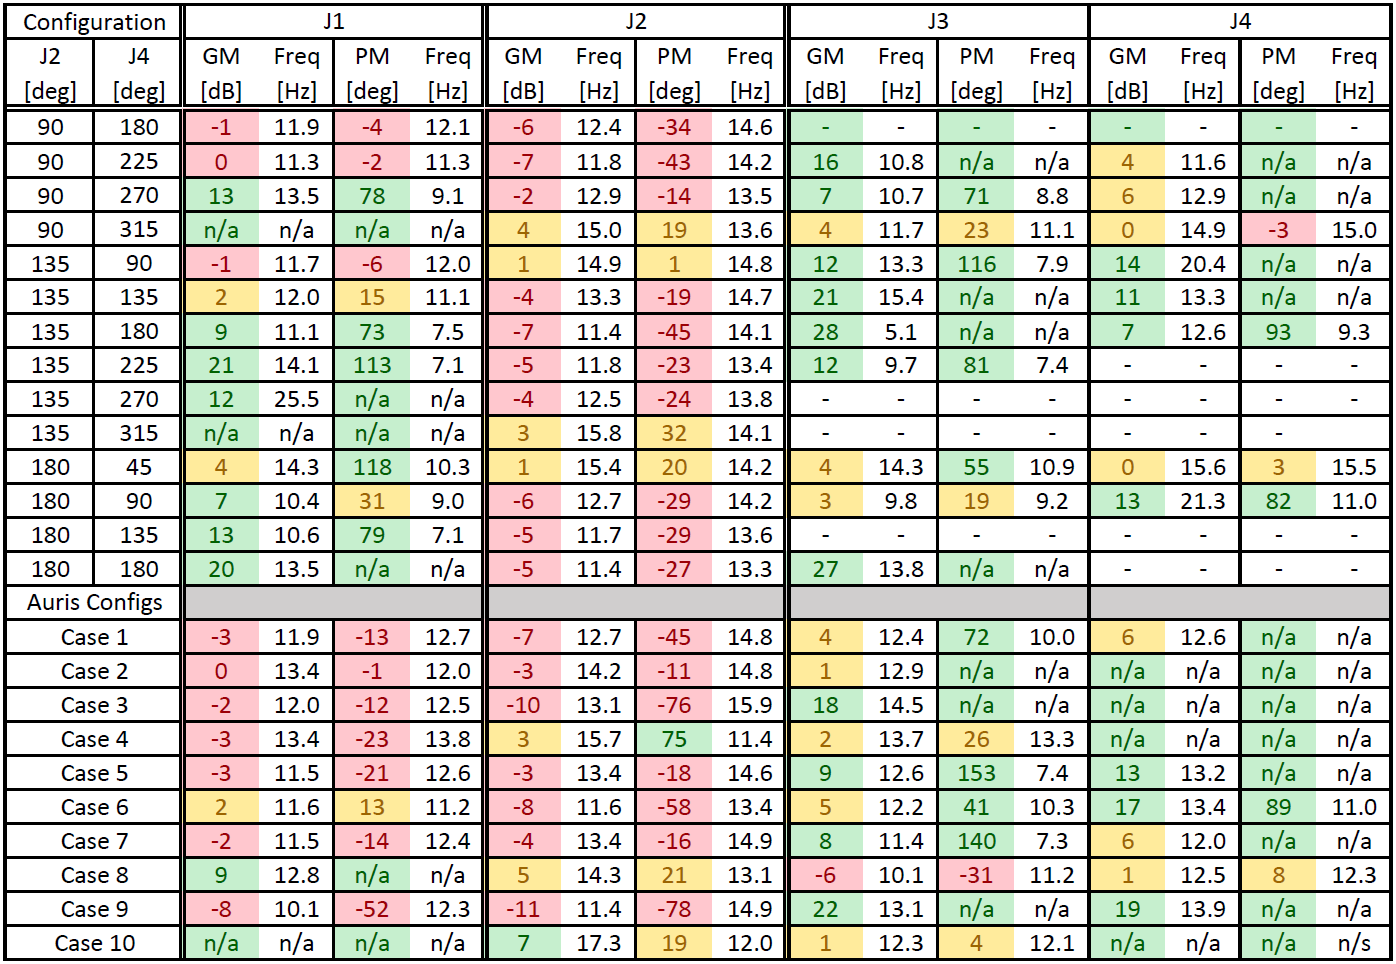
\includegraphics[width=1\textwidth]{./images/SAtable.pdf}%
		%		\includegraphics[width=0.5\textwidth]{./images/test_setup_2.JPG}%
		% test_setup
		\label{table:SAtable}
	\end{table}


\subsection{Concerns about current method and results}
\begin{itemize}
	\item Datalog
	
	Slow refresh rates and difficulty to synchronize data represent a important factor of error. Getting better refresh rate, more data outputs and a deeper analysis to synchronize data would greatly enhance confidence in the data collected and results obtained. 
	
	\item Sine-swept in position
	
	The limitation to the use of a sine-swept in position does not allows the deactivation of that particular loop. The position loop is therefore affecting the behavior of the system and reduce confidence in the results obtained for the torque loop. The capacity to activate and deactivate both loop separately and dive torque inputs to the corresponding loop would be a significant enhancement. 
    
    \item Data validation
    
    Very little data validation has been not yet. This is an important process to ensure collected data and results represent the behavior of the system.
    
	\item Analysis tools
	
	Further study of the analysis tools, mainly MATLAB data analysis functions, would be preferable to validate results.
	
\end{itemize}

%\section{Possible amelioration and future works}
%\subsection{MS5-6 Rev2c possible improvements}
Possible improvements on the MS5-6~Rev2c:
%\subsubsection{Possible improvements}
\begin{itemize}
	\item Torque compensator would benefit of more tuning in regards to the former stability analysis.
	\item Firmware development for new outputs and faster refresh rates would help to perform frequency responses.
	\item PID would benefit of more tuning, namely by performing frequency responses.
	\item PID could be replaced by a more general compensator similar to the one used on torque.
\end{itemize} 

\subsection{MS7}
MS7 arms will have a different architecture compared to MS5-6~Rev2c. Therefore, work done on Rev2c may no be valuable for MS7. Major differences, which address a lot of limitations of Rev2c arms, are:
\begin{itemize}
	\item Second encoder on the output size may allow vibration damping. If this is the case, torque feedback compensation might be no longer needed.
	\item Torque loop will be ran at 1~kHz.
	\item Use of current, velocity and position loops.
	\item More rigid links.
	\item Faster chips and better communication will allow faster data acquisition of any needed data.
\end{itemize}


\subsection{Future works}
Future works currently in scope for vibration damping and controller loops tuning are: 
\begin{itemize}
	\item Development of standard methods for controller tuning and stability analysis for MS7.
	\item Give specific requirements to firmware team in terms of loops design, rates and datalogging for MS7.
	\item Perform better characterization of Rev2c actuators and arms and develop a simulation model.
	\item Update of the simulation model to MS7 specifications to speed up controller design.
\end{itemize}

%\subsubsection{Design changes} 
%The current torque feedback filter has been fixed for MS 5-6. However design improvements can continue for research purposes which might
%be useful for MS 7. It is to be noted however that, MS 7 will have very different control architechture than MS 5-6 and results will not 
%directly feed into it.


%\subsection{MS 7}
%\begin{itemize}
%	\item With the encoder on the output side, vibrations due to the harmonic drive can possibily be damped by the position loop itself.
%	If so, torque feedback compensation might be no longer needed.  
%	\item Simulations - MS 7 hardware will not be available for near future. Simulating Harmonic Drive vibrations, with encoder on the output side
%	will help speed up control design and stability analysis. 
%\end{itemize}

%\section{Conclusion}
%Torque feedback as it is now in MS5-6~Rev2c arms helps dampen vibration. Even though torque feedback does not suppress completely small vibration, it definitely helps to contain vibration within a certain range and reduce settling time. However, from the current stability analysis, torque open loop margins are negative for an important part of the workspace. No instability has been observed in operation, which means the controller, the two closed loops together, position and torque, is stable.

There is a couple of possible ameliorations that could be done on MS5-6~Rev2c arms. However, this work may not be reusable for MS7. The focus now is to progress on MS7 controller concept and ensure good methods will be implemented for tuning and stability analysis. Concept review should be presented soon for MS7, while actuators and the base are currently in design phase, to make sure that control requirements will be met in regards of the hardware and the firmware.

%\newpage

%\section{Ongoing Work}
%\input{ongoing.tex}

%\newpage

%\section{Torque Feedback Tuning}
%\input{torqueFeedback.tex}

%\newpage

%\section{Admittance mode, faults and other warnings}
%\input{warnings.tex}

%\newpage

%\section{Short term objectives}
%\input{futureWorks.tex}

%\newpage


%\section*{Revisions}
%
%\begin{tabular}{|m{0.2\textwidth}|m{0.7\textwidth}|}
%  \hline
%  Date & Changes                                                              \\ \hline
%  2016/01/28 & Initial Version                                                \\ \hline
%\end{tabular}
%
\end{document}
